\documentclass{standalone}
\usepackage{tikz}
\usetikzlibrary{patterns, positioning}
\usepackage[sfdefault]{ClearSans} %% option 'sfdefault' activates Clear Sans as the default text font
\usepackage[T1]{fontenc}

\begin{document}
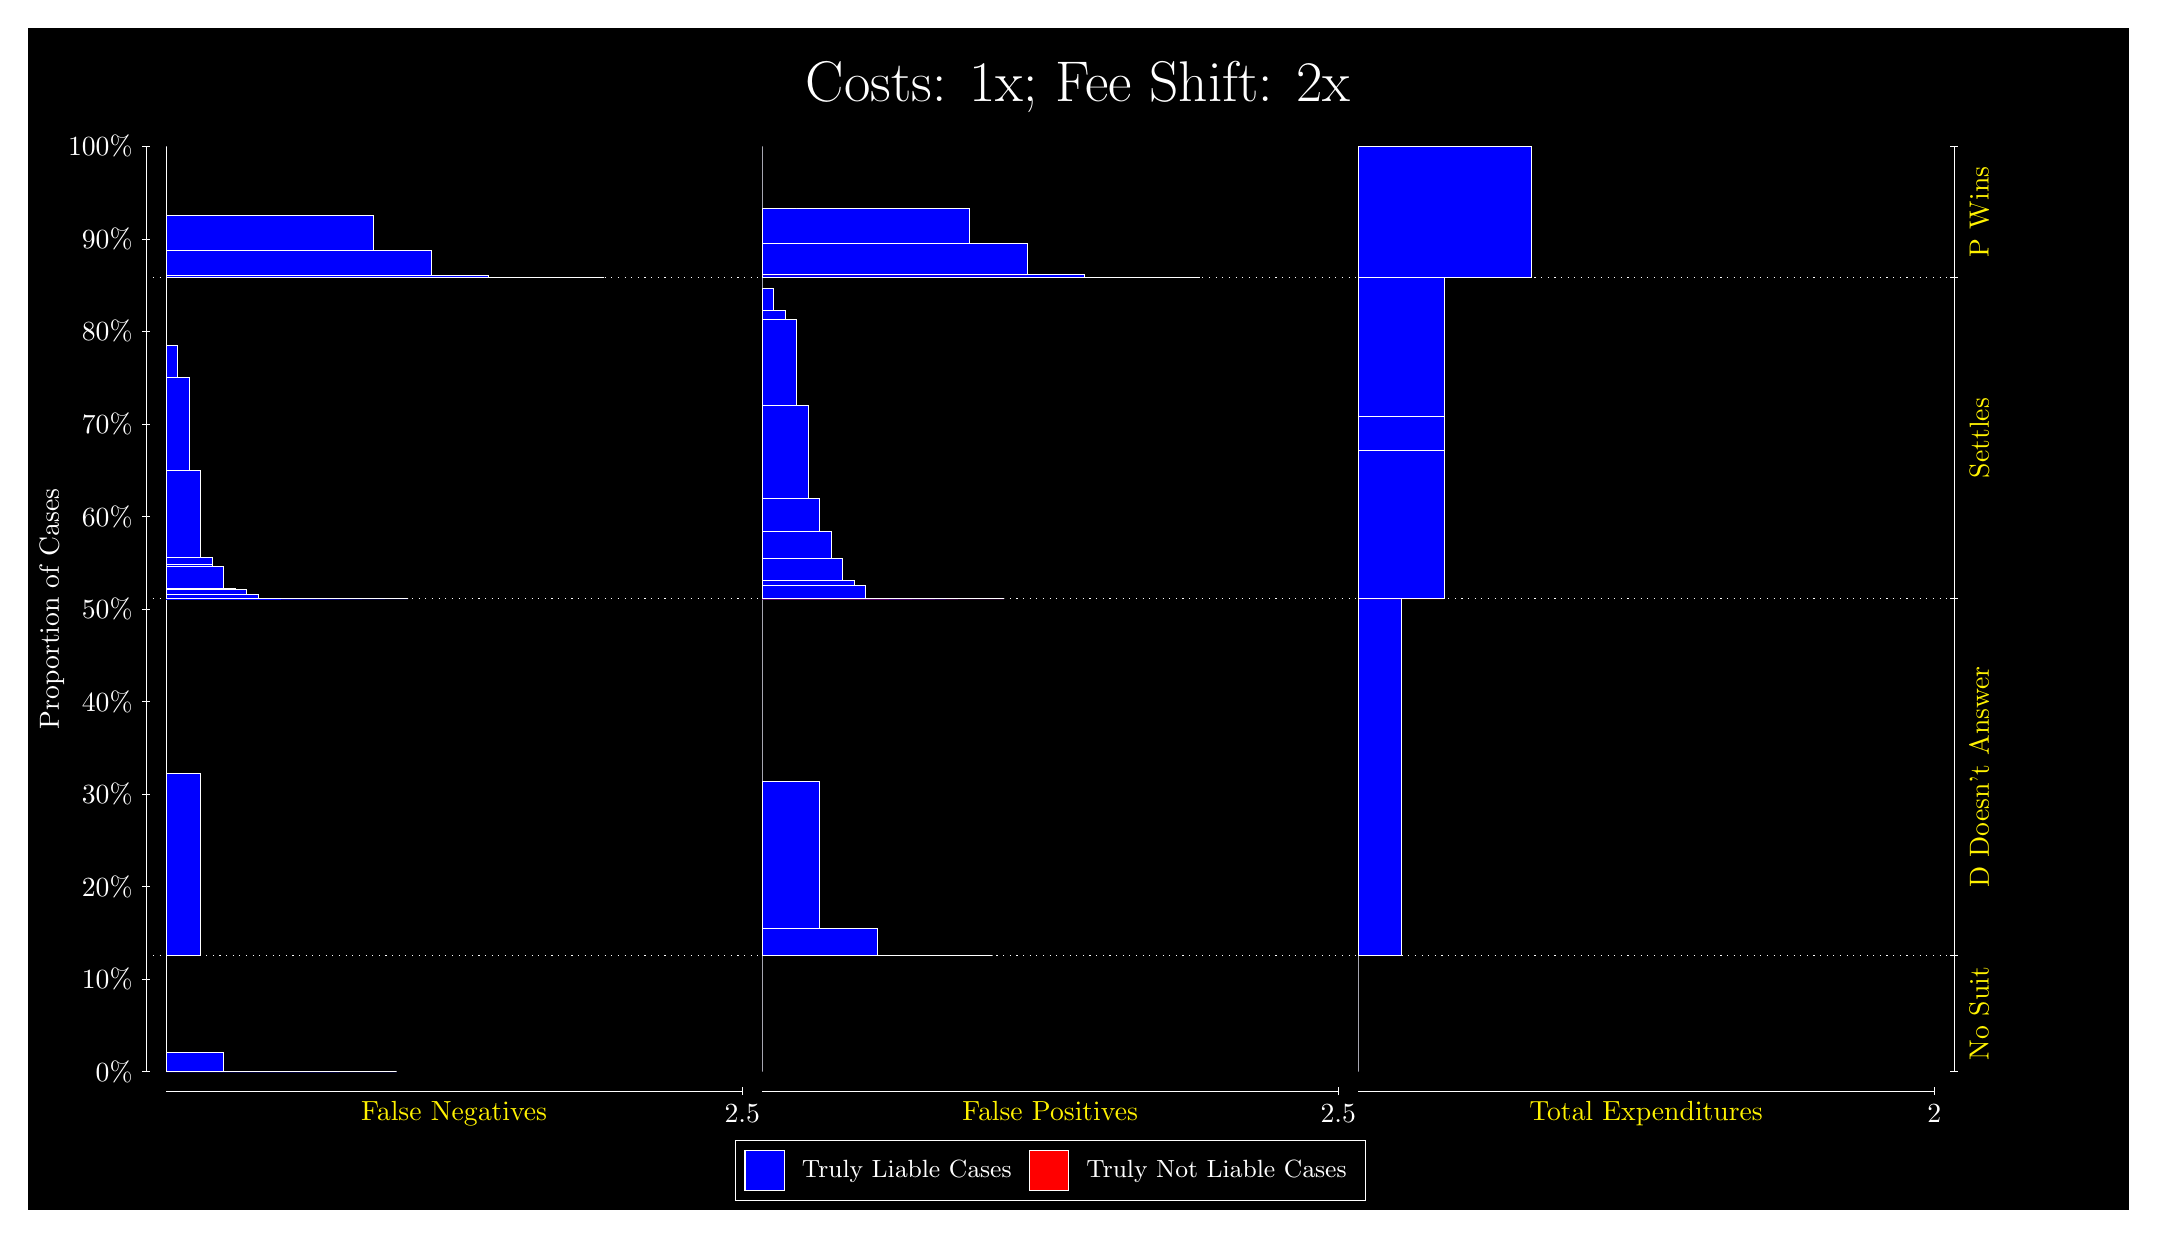
\begin{tikzpicture}
\draw[fill=black] (0,0) rectangle (26.667,15);
\draw[text=white] (0,13.5) rectangle (26.667,15) node[midway] {\huge Costs: 1x; Fee Shift: 2x};
\draw[white, very thin] (1.5,1.75) -- (1.5,13.5);
\node[rotate=90, text=white, anchor=center] at (0.3, 7.625) {Proportion of Cases};
\draw[white, very thin] (1.45,1.75) -- (1.55,1.75);
\node[text=white, anchor=east] at (1.45, 1.75) {0\%};
\draw[white, very thin] (1.45,2.925) -- (1.55,2.925);
\node[text=white, anchor=east] at (1.45, 2.925) {10\%};
\draw[white, very thin] (1.45,4.1) -- (1.55,4.1);
\node[text=white, anchor=east] at (1.45, 4.1) {20\%};
\draw[white, very thin] (1.45,5.275) -- (1.55,5.275);
\node[text=white, anchor=east] at (1.45, 5.275) {30\%};
\draw[white, very thin] (1.45,6.45) -- (1.55,6.45);
\node[text=white, anchor=east] at (1.45, 6.45) {40\%};
\draw[white, very thin] (1.45,7.625) -- (1.55,7.625);
\node[text=white, anchor=east] at (1.45, 7.625) {50\%};
\draw[white, very thin] (1.45,8.8) -- (1.55,8.8);
\node[text=white, anchor=east] at (1.45, 8.8) {60\%};
\draw[white, very thin] (1.45,9.975) -- (1.55,9.975);
\node[text=white, anchor=east] at (1.45, 9.975) {70\%};
\draw[white, very thin] (1.45,11.15) -- (1.55,11.15);
\node[text=white, anchor=east] at (1.45, 11.15) {80\%};
\draw[white, very thin] (1.45,12.325) -- (1.55,12.325);
\node[text=white, anchor=east] at (1.45, 12.325) {90\%};
\draw[white, very thin] (1.45,13.5) -- (1.55,13.5);
\node[text=white, anchor=east] at (1.45, 13.5) {100\%};

\draw[white, very thin] (24.457,1.75) -- (24.457,13.5);
\draw[white, very thin] (24.407,1.75) -- (24.507,1.75);
\node[anchor=west] at (24.407, 1.75) {};
\draw[white, very thin] (24.407,3.2238) -- (24.507,3.2238);
\node[anchor=west] at (24.407, 3.2238) {};
\draw[white, very thin] (24.407,7.7554) -- (24.507,7.7554);
\node[anchor=west] at (24.407, 7.7554) {};
\draw[white, very thin] (24.407,11.836) -- (24.507,11.836);
\node[anchor=west] at (24.407, 11.836) {};
\draw[white, very thin] (24.407,13.5) -- (24.507,13.5);
\node[anchor=west] at (24.407, 13.5) {};

\draw[white, very thin, fill=blue] (1.75,1.75) rectangle (4.6775,1.75);
\draw[white, very thin, fill=blue] (1.75,1.75) rectangle (3.9457,1.75);
\draw[white, very thin, fill=blue] (1.75,1.75) rectangle (3.2138,1.7521);
\draw[white, very thin, fill=blue] (1.75,1.7521) rectangle (2.4819,1.9913);
\draw[white, very thin, fill=red] (1.75,1.9913) rectangle (1.75,1.9913);
\draw[white, very thin, fill=blue] (1.75,1.9913) rectangle (1.75,3.2238);
\draw[white, very thin, fill=blue] (1.75,3.2238) rectangle (2.1891,5.5397);
\draw[white, very thin, fill=red] (1.75,5.5397) rectangle (1.75,5.5397);
\draw[white, very thin, fill=blue] (1.75,5.5397) rectangle (1.75,7.7554);
\draw[white, very thin, fill=blue] (1.75,7.7554) rectangle (4.8239,7.7554);
\draw[white, very thin, fill=blue] (1.75,7.7554) rectangle (4.5312,7.7554);
\draw[white, very thin, fill=blue] (1.75,7.7554) rectangle (4.2384,7.7554);
\draw[white, very thin, fill=blue] (1.75,7.7554) rectangle (4.092,7.7554);
\draw[white, very thin, fill=blue] (1.75,7.7554) rectangle (3.9457,7.7554);
\draw[white, very thin, fill=blue] (1.75,7.7554) rectangle (3.7993,7.7554);
\draw[white, very thin, fill=blue] (1.75,7.7554) rectangle (3.6529,7.7554);
\draw[white, very thin, fill=blue] (1.75,7.7554) rectangle (3.5065,7.7554);
\draw[white, very thin, fill=blue] (1.75,7.7554) rectangle (3.3602,7.7554);
\draw[white, very thin, fill=blue] (1.75,7.7554) rectangle (3.2138,7.7559);
\draw[white, very thin, fill=blue] (1.75,7.7559) rectangle (3.0674,7.7559);
\draw[white, very thin, fill=blue] (1.75,7.7559) rectangle (3.0674,7.7561);
\draw[white, very thin, fill=blue] (1.75,7.7561) rectangle (2.921,7.8151);
\draw[white, very thin, fill=blue] (1.75,7.8151) rectangle (2.7746,7.8742);
\draw[white, very thin, fill=blue] (1.75,7.8742) rectangle (2.6283,7.8743);
\draw[white, very thin, fill=blue] (1.75,7.8743) rectangle (2.6283,7.8899);
\draw[white, very thin, fill=blue] (1.75,7.8899) rectangle (2.4819,8.1725);
\draw[white, very thin, fill=blue] (1.75,8.1725) rectangle (2.3355,8.1901);
\draw[white, very thin, fill=blue] (1.75,8.1901) rectangle (2.3355,8.2847);
\draw[white, very thin, fill=blue] (1.75,8.2847) rectangle (2.1891,9.3806);
\draw[white, very thin, fill=blue] (1.75,9.3806) rectangle (2.0428,10.562);
\draw[white, very thin, fill=blue] (1.75,10.562) rectangle (1.8964,10.566);
\draw[white, very thin, fill=blue] (1.75,10.566) rectangle (1.8964,10.978);
\draw[white, very thin, fill=red] (1.75,10.978) rectangle (1.75,10.978);
\draw[white, very thin, fill=blue] (1.75,10.978) rectangle (1.75,11.836);
\draw[white, very thin, fill=blue] (1.75,11.836) rectangle (7.3123,11.836);
\draw[white, very thin, fill=blue] (1.75,11.836) rectangle (6.5805,11.836);
\draw[white, very thin, fill=blue] (1.75,11.836) rectangle (5.8486,11.856);
\draw[white, very thin, fill=blue] (1.75,11.856) rectangle (5.1167,12.178);
\draw[white, very thin, fill=blue] (1.75,12.178) rectangle (4.3848,12.622);
\draw[white, very thin, fill=blue] (1.75,12.622) rectangle (3.6529,12.622);
\draw[white, very thin, fill=blue] (1.75,12.622) rectangle (3.0674,12.622);
\draw[white, very thin, fill=blue] (1.75,12.622) rectangle (2.921,12.622);
\draw[white, very thin, fill=blue] (1.75,12.622) rectangle (2.3355,12.622);
\draw[white, very thin, fill=red] (1.75,12.622) rectangle (1.75,12.622);
\draw[white, very thin, fill=blue] (1.75,12.622) rectangle (1.75,13.5);
\draw[white, very thin, fill=red] (9.3189,1.75) rectangle (9.3189,1.75);
\draw[white, very thin, fill=blue] (9.3189,1.75) rectangle (9.3189,3.2238);
\draw[white, very thin, fill=red] (9.3189,3.2238) rectangle (12.246,3.2238);
\draw[white, very thin, fill=blue] (9.3189,3.2238) rectangle (12.246,3.2238);
\draw[white, very thin, fill=blue] (9.3189,3.2238) rectangle (11.515,3.2265);
\draw[white, very thin, fill=blue] (9.3189,3.2265) rectangle (10.783,3.5736);
\draw[white, very thin, fill=blue] (9.3189,3.5736) rectangle (10.051,5.4395);
\draw[white, very thin, fill=blue] (9.3189,5.4395) rectangle (9.3189,7.7554);
\draw[white, very thin, fill=red] (9.3189,7.7554) rectangle (12.393,7.7554);
\draw[white, very thin, fill=blue] (9.3189,7.7554) rectangle (12.393,7.7554);
\draw[white, very thin, fill=red] (9.3189,7.7554) rectangle (11.807,7.7554);
\draw[white, very thin, fill=blue] (9.3189,7.7554) rectangle (11.807,7.7554);
\draw[white, very thin, fill=blue] (9.3189,7.7554) rectangle (11.661,7.7554);
\draw[white, very thin, fill=red] (9.3189,7.7554) rectangle (11.515,7.7554);
\draw[white, very thin, fill=blue] (9.3189,7.7554) rectangle (11.515,7.7554);
\draw[white, very thin, fill=red] (9.3189,7.7554) rectangle (11.222,7.7554);
\draw[white, very thin, fill=blue] (9.3189,7.7554) rectangle (11.222,7.7554);
\draw[white, very thin, fill=blue] (9.3189,7.7554) rectangle (11.075,7.7554);
\draw[white, very thin, fill=red] (9.3189,7.7554) rectangle (10.929,7.7554);
\draw[white, very thin, fill=blue] (9.3189,7.7554) rectangle (10.929,7.7601);
\draw[white, very thin, fill=blue] (9.3189,7.7601) rectangle (10.783,7.7603);
\draw[white, very thin, fill=red] (9.3189,7.7603) rectangle (10.636,7.7603);
\draw[white, very thin, fill=blue] (9.3189,7.7603) rectangle (10.636,7.931);
\draw[white, very thin, fill=blue] (9.3189,7.931) rectangle (10.49,7.9894);
\draw[white, very thin, fill=red] (9.3189,7.9894) rectangle (10.344,7.9894);
\draw[white, very thin, fill=blue] (9.3189,7.9894) rectangle (10.344,8.2671);
\draw[white, very thin, fill=blue] (9.3189,8.2671) rectangle (10.197,8.6131);
\draw[white, very thin, fill=red] (9.3189,8.6131) rectangle (10.051,8.6131);
\draw[white, very thin, fill=blue] (9.3189,8.6131) rectangle (10.051,9.03);
\draw[white, very thin, fill=blue] (9.3189,9.03) rectangle (9.9044,10.211);
\draw[white, very thin, fill=blue] (9.3189,10.211) rectangle (9.758,11.307);
\draw[white, very thin, fill=blue] (9.3189,11.307) rectangle (9.6116,11.419);
\draw[white, very thin, fill=blue] (9.3189,11.419) rectangle (9.4652,11.702);
\draw[white, very thin, fill=blue] (9.3189,11.702) rectangle (9.3189,11.836);
\draw[white, very thin, fill=red] (9.3189,11.836) rectangle (14.881,11.836);
\draw[white, very thin, fill=blue] (9.3189,11.836) rectangle (14.881,11.836);
\draw[white, very thin, fill=red] (9.3189,11.836) rectangle (14.149,11.836);
\draw[white, very thin, fill=blue] (9.3189,11.836) rectangle (14.149,11.837);
\draw[white, very thin, fill=red] (9.3189,11.837) rectangle (13.417,11.837);
\draw[white, very thin, fill=blue] (9.3189,11.837) rectangle (13.417,11.869);
\draw[white, very thin, fill=red] (9.3189,11.869) rectangle (12.686,11.869);
\draw[white, very thin, fill=blue] (9.3189,11.869) rectangle (12.686,12.275);
\draw[white, very thin, fill=blue] (9.3189,12.275) rectangle (11.954,12.712);
\draw[white, very thin, fill=blue] (9.3189,12.712) rectangle (11.222,12.714);
\draw[white, very thin, fill=blue] (9.3189,12.714) rectangle (10.49,12.714);
\draw[white, very thin, fill=red] (9.3189,12.714) rectangle (9.9044,12.714);
\draw[white, very thin, fill=blue] (9.3189,12.714) rectangle (9.9044,12.714);
\draw[white, very thin, fill=blue] (9.3189,12.714) rectangle (9.758,12.714);
\draw[white, very thin, fill=red] (9.3189,12.714) rectangle (9.3189,12.714);
\draw[white, very thin, fill=blue] (9.3189,12.714) rectangle (9.3189,13.5);
\draw[white, very thin, fill=red] (16.888,1.75) rectangle (16.888,1.75);
\draw[white, very thin, fill=blue] (16.888,1.75) rectangle (16.888,3.2238);
\draw[white, very thin, fill=red] (16.888,3.2238) rectangle (17.437,3.2238);
\draw[white, very thin, fill=blue] (16.888,3.2238) rectangle (17.437,7.7554);
\draw[white, very thin, fill=red] (16.888,7.7554) rectangle (17.986,7.7554);
\draw[white, very thin, fill=blue] (16.888,7.7554) rectangle (17.986,9.642);
\draw[white, very thin, fill=red] (16.888,9.642) rectangle (17.986,9.642);
\draw[white, very thin, fill=blue] (16.888,9.642) rectangle (17.986,10.07);
\draw[white, very thin, fill=red] (16.888,10.07) rectangle (17.986,10.07);
\draw[white, very thin, fill=blue] (16.888,10.07) rectangle (17.986,11.836);
\draw[white, very thin, fill=red] (16.888,11.836) rectangle (19.083,11.836);
\draw[white, very thin, fill=blue] (16.888,11.836) rectangle (19.083,13.5);
\draw[white, dotted] (1.5,3.2238) -- (24.457,3.2238);
\draw[white, dotted] (1.5,7.7554) -- (24.457,7.7554);
\draw[white, dotted] (1.5,11.836) -- (24.457,11.836);
\draw[white, very thin] (1.75,1.5) -- (9.0689,1.5);
\node[text=yellow, anchor=north] at (5.4094, 1.5) {False Negatives};
\draw[white, very thin] (9.0689,1.45) -- (9.0689,1.55);
\node[text=white, anchor=north] at (9.0689, 1.45) {2.5};

\draw[white, very thin] (9.3189,1.5) -- (16.638,1.5);
\node[text=yellow, anchor=north] at (12.978, 1.5) {False Positives};
\draw[white, very thin] (16.638,1.45) -- (16.638,1.55);
\node[text=white, anchor=north] at (16.638, 1.45) {2.5};

\draw[white, very thin] (16.888,1.5) -- (24.207,1.5);
\node[text=yellow, anchor=north] at (20.547, 1.5) {Total Expenditures};
\draw[white, very thin] (24.207,1.45) -- (24.207,1.55);
\node[text=white, anchor=north] at (24.207, 1.45) {2};

\node[text=yellow, centered, rotate=90] at (24.777, 2.4869) {No Suit};
\node[text=yellow, centered, rotate=90] at (24.777, 5.4896) {D Doesn't Answer};
\node[text=yellow, centered, rotate=90] at (24.777, 9.7958) {Settles};
\node[text=yellow, centered, rotate=90] at (24.777, 12.668) {P Wins};

\draw (12.978300999999998,1.5) node[draw=none] (baseCoordinate) {};
\begin{scope}[align=center]
        \matrix[scale=0.5, draw=white, below=0.5cm of baseCoordinate, nodes={draw}, column sep=0.1cm]{
            \node[rectangle, draw, minimum width=0.5cm, minimum height=0.5cm, fill=blue] {}; &
            \node[draw=none, font=\small, text=white] (B) {Truly Liable Cases}; &
            \node[rectangle, draw, minimum width=0.5cm, minimum height=0.5cm, fill=red] {}; &
            \node[draw=none, font=\small, text=white] (B) {Truly Not Liable Cases}; \\
            };
\end{scope}

\end{tikzpicture}
\end{document}